\documentclass{article}

\usepackage[utf8]{inputenc}
\usepackage{amsmath}
\usepackage{amsfonts}
\usepackage[final]{pdfpages} 
\usepackage{cases}
\usepackage{soul}
\usepackage{pict2e}
\usepackage{graphicx}
\usepackage{minted}
\usepackage[final]{pdfpages} 

\usepackage[top=2.25cm, bottom=2.25cm, left=2cm, right=2cm]{geometry}
\newcommand{\g}[2]{g_{#1}^{#2}}
\newcommand{\f}[2]{f_{#1}^{#2}}
\newcommand{\Min}[2]{ {#1} \wedge {#2} }
\newcommand{\undemi}{ \frac{1}{2} }
\newcommand{\proba}[3]{ \mathbb{P}_{X_0=#1} (#3 | S_0=#2) }
\newcommand{\comment}[1]{}
\newcommand{\IMG}[1] { \includegraphics[scale=0.35]{img/#1.png} }
\newcommand{\IMGG}[1] { \includegraphics[scale=0.5]{img/#1.png} }

\newcommand{\IMGC}[1] {
\begin{center} \includegraphics[scale=0.5]{img/#1.png} \end{center}
 }


\begin{document}

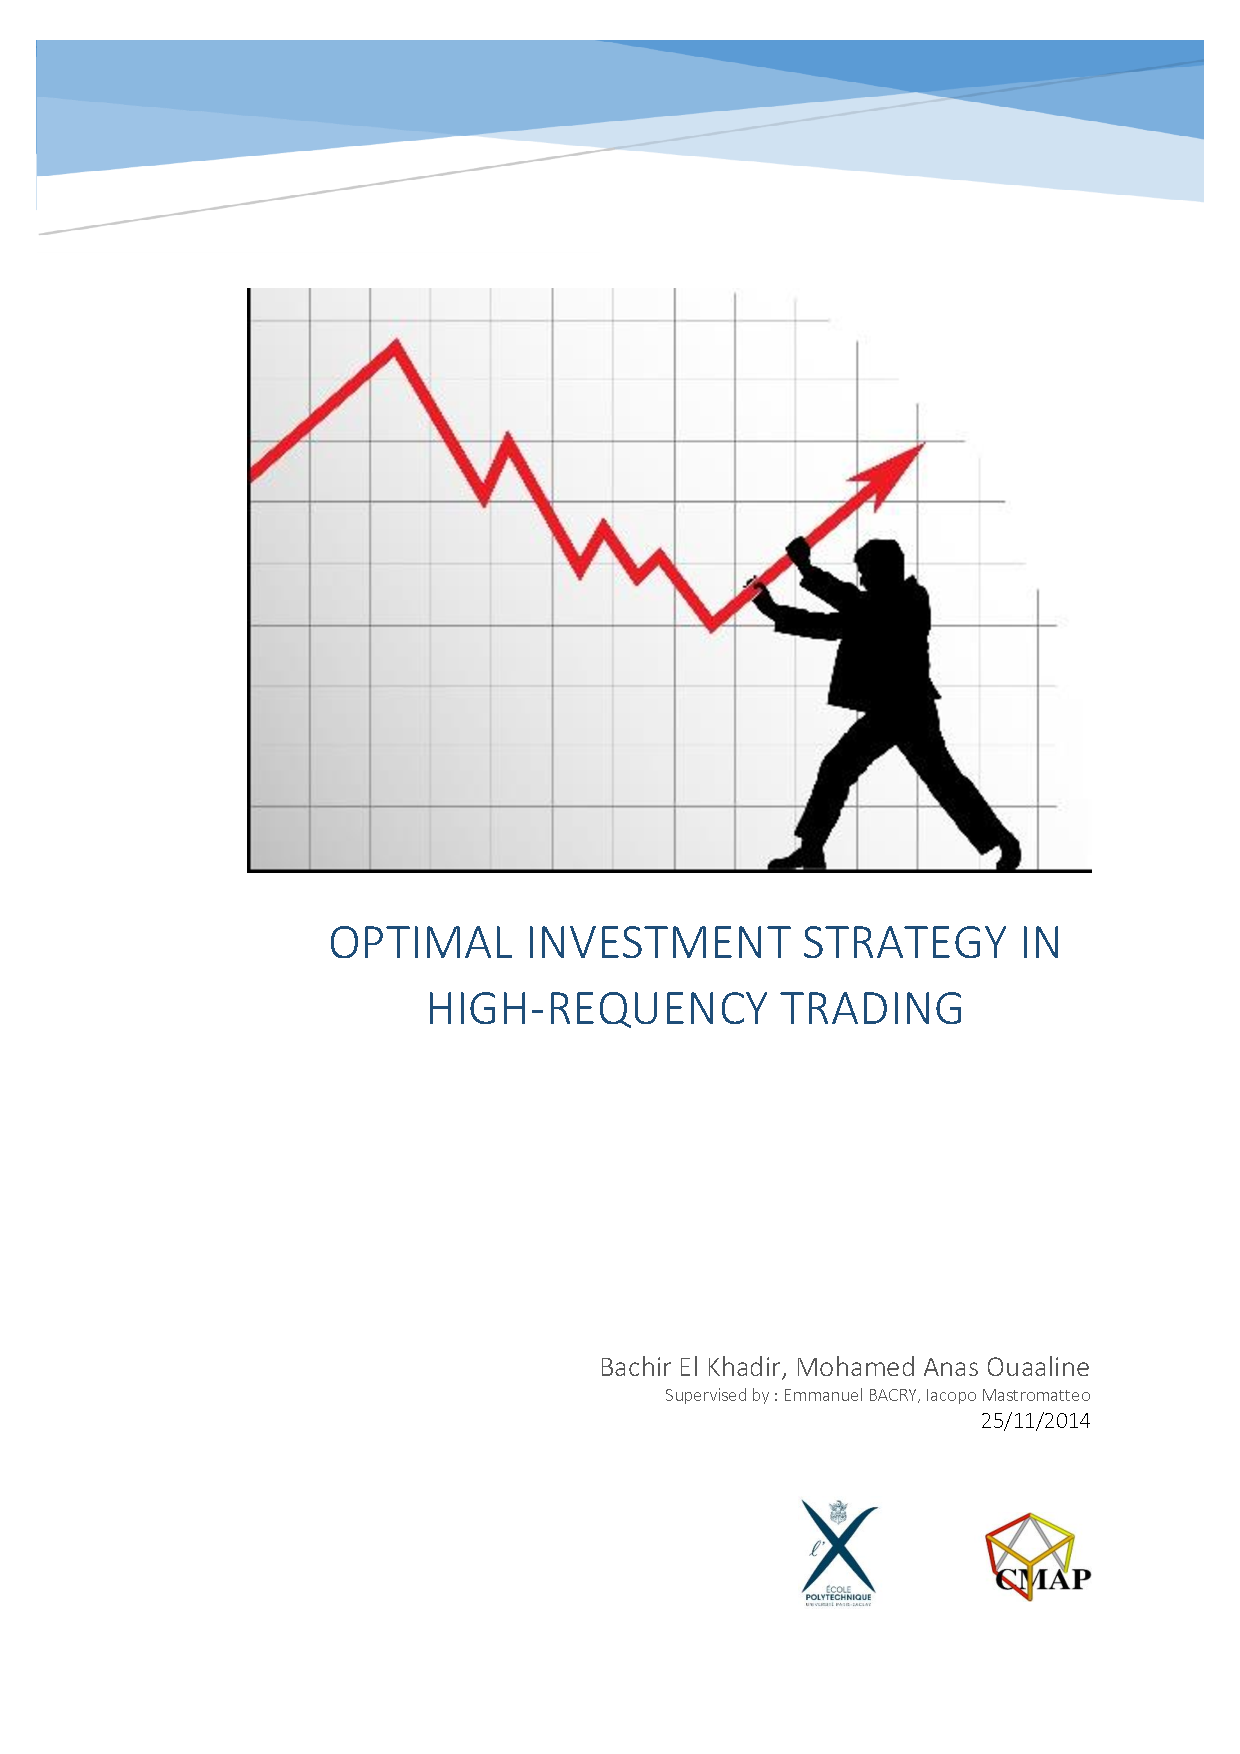
\includepdf{pagedegarde.pdf}

\begin{abstract}
Given the state of an order book, we want to place purchase orders. Through this document, we try to define an efficient and optimal strategy in order to reduce the cost of such orders. Since it is quite complex to define this kind of strategies, we focus on the case where we have only one purchase order to make and a time horizon before which the trade must be executed. We have the choice between executing the order directly (market order), or placing a limit order. Since we are never sure that a limit order will be executed, we have to remove it after a certain time k and place a market order instead at the best offer available. Notice that the case where $k = 0$ is when a market order is executed immediately.
The cost related to these kind of strategies can be of two types:

\begin{itemize}
	\item Cost related to the spread when executing a market order.
	\item Cost related to the uncertainty of future price movements that we denote $c$.
\end{itemize}
While the first is easily measurable, the second is dependent on many factors: volatility of the market, the risk aversion of the trader... 
We will discuss this issue further in the following sections.
The goal of this document becomes:
\begin{quote}
\textit{Given the state of an order book and a single purchase order we want to make, what it is the best choice of $k$ to minimize the cost of the trade  ?}
\end{quote}
\end{abstract}

\tableofcontents

\newpage



\section{The model and its dynamic}
Let us present the basic model which our study is based on.

\subsection{The model}
The order book is represented by its best ask and bid queues. The state of the limit order book is represented by :
\begin{itemize}
\item the bid price $ s_{t}^{a} $ and the ask price $ s_{t}^{b} $ 
\item the size of the bid queue $ q_{t}^{a} $ representing the outstanding limit buy orders at the bid, and 
\item the size of the ask queue $ q_{t}^{b} $ representing the outstanding limit sell orders at the ask 
\end{itemize}
The bid and ask prices are multiples of the tick size $\delta = s_{t}^{a} - s_{t}^{b}$ which we consider constant.
The state of the limit order book is thus described by the triplet $X_{t} = (s_{t}^{b}, q_{t}^{b}, q_{t}^{a})$ which takes values in the discrete state space $\delta \mathbb{Z} \times \mathbb{N}^{2} $. With no loss of generality, we can assume that  :
\begin{equation}
\delta = 1
\end{equation}
We assume that orders arriving at the best bid/ask follow a poissonian process and are all of the same size $1$:
\begin{itemize}
	\item A market/cancelation order arriving at the $q_t^a$ (resp $q_t^b$) reduces its size by 1 if it is not empty
	\item A limit order arriving at the $q_t^a$ (resp $q_t^b$) adds 1 to its size 
\end{itemize}
Therefore $q_t^a$ and $q_t^b$ follow a birth/death process.
We denote :
\begin{itemize}
\item $(\tau_i)_{_{i \geq 1}}$ the sequence of random variables  which stands for times between successive price changes. \footnote { Cont and Larrard's article presents an expression for the cumulative distribution function of each $\tau_i$. }
\item $(X_i)_{_{i \geq 1}}$ the successive moves in the price. Note that according to our hypothesis ($\delta = 1$) : $X_i \in \{-1,1\}$ .
\item $(S_k)_{_{i \geq 0}}$ the cumulative moves in the price after the $n^{th}$ change, ie $S_n = \sum{1 \leq i \leq n } X_i$. \footnote{ see Annexe \ref{loi_S} for the generating function of $S_n$ }  
\end{itemize}

\subsection{The dynamic}

The state  of the order book is modified by order book events. When the bid (resp. ask) queue is empty, the price moves down (resp. up), and $(q_t^a, q_t^b)$ (resp.$ (q_t^b, q_t^a)$ is generated from a distribution $f(x, y) \mathrm{d}x \mathrm{d}y $ (resp. $\tilde f(x, y) \mathrm{d}x \mathrm{d}y $) independently from the rest of the historical variables.
The next image is a graphical representation of $f$ when estimated from historical data.

\IMGC{hist_f}

This property give the market a markovian property: the new state of the market after a price move does only depend on the direction of this move.
Therefore,  $(X_i)_{_{i \geq 0}}$ is markov process such as :
\begin{itemize}
\item $\forall \, n\geq0 \quad X_{n} \in \{-1,1\} $ 
\item $\forall \, i\geq0 \quad\ \mathbb{P}( X_{i+1}=1 | X_i=1 ) = \mathbb{P}( X_{i+1}=-1 | X_i=-1 ) = p = 1-q$
\end{itemize}
Given the symmetry of the market, we may assume that $f(x, y) = \tilde f(y, x)$. This assumption makes the process $(\tau_i)_i$ a sequence of IID random variables independent from $(X_i)_i$.

\section{The optimization problem}
Recall how our strategy works:
\begin{itemize}
	\item A limit order is placed at t=0 at the best bid.
	\item after some time $T = \sum_{i \leq k} \tau_i$, if the order is not executed, we cancel it and make a market order at the ask side.
\end{itemize}
$k$ is the parameter of the strategy we seek to optimize. It stands for the maximum number of moves in price we are willing to wait for. Let's call it $\text{Strategy}(k)$ .
Let N be the first time where the sequence $(S_{n})_{n\geq0}$  achieves $-1$. Thereby :
$$ N= \inf \{ n\geq0 , S_{n}=-1   \} $$
Finally, we denote $c_{wait}$ the waiting cost per unit of time.
The problem could be seen as a minimization problem  :
\begin{equation}
 \min\limits_{k \in \mathbb{N}} \quad f(k) := \min\limits_{k \in \mathbb{N}} \quad \mathbb{E}\,\left[ \sum_{i=1}^{\Min k N}\tau_i c_{wait} + (S_{\Min k N)}+1)\delta\right]
\end{equation}
We shall notice that $(\tau_i)_{(i>0)}$ are assumed to be independent. The are also assumed to be independent of $N$.
Thus we can rewrite $f$ and the problem becomes : 
\begin{equation}
 \min\limits_{k \in \mathbb{N}} \quad f(k)= \min\limits_{k \in \mathbb{N}} \quad \mathbb{E}\,\left[ ({\Min k N})  \mathbb{E}(\tau) c_{wait} + (S_{\Min k N}+1) \right]
\end{equation}
Since $\mathbb{E}(\tau)$ is a constant we can denote
$c = \mathbb{E}(\tau) c_{wait}$ which is the waiting cost per price move. And the minimization problem finally becomes :
\begin{equation}
 \min\limits_{k \in \mathbb{N}} \quad f(k)= \min\limits_{k \in \mathbb{N}} \quad c \mathbb{E}\,\left[ {\Min k N}\right]   +  \mathbb{E}\,\left[S_{\Min k N}\right] +1
\end{equation}
In order to solve this problem we need to do 2 different calculations :
\begin{itemize}
\item $\mathbb{E}\,\left[ {\Min k N}\right]$ : we are going to explicitly calculate the Law N
\item $\mathbb{E}\,\left[S_{\Min k N}\right]$ : since $S_i$ and $N$ are not independent, the law is quite hard to be explicitly calculated. Consequently, we are going to use a Monte-Carlo Algorithm.
\end{itemize}
\textbf{The parameter c:}\\
In the previous section we have denoted :
$$
	c = \mathbb{E}(\tau) c_{wait}
$$
It is an exogenous parameter which has to manually fixed. We notice that through its definition $c$ depends on $\mathbb{E}(\tau)$ which is the average time between two moves in the price. However we can be more accurate and see that it also depends on the volatility of the market and the operator's risk aversion. We also notice that $c$ needs to be lower than the thick $\delta$ otherwise it is not interesting to wait for a move in the price.
Thus we came up with the following remarks.
\begin{itemize}
\item $c = \mathbb{E}(\tau) F(\sigma,v,r)$ where $ \mathbb{E}(\tau)$ is the average time between two moves in the price, $\sigma$ is the market volatility, $v$ is the operator's risk aversion and $r$ is some unknown parameters. 
\item $c<\delta$ where $\delta$ is the thick.
\item $c$ is increasing in $\sigma$ : The more the market is volatile the more it risky is to wait.
\item $c$ is increasing in $v$ : The more the operator is averse to risk the more likely he is to over-rate the waiting cost. 
\end{itemize}
In our model we assume that $\mathbb{E}(\tau) , \sigma, v
$ and $r$ do not depends on $k$.

\newpage
\section{Solving the minimization problem}
\subsection{First time of reach for a sum of a Markov chain}
In this section we address the issue of finding the law of the variable $N$. Let us define the  probability-generating function of $N$ such as :
$$ g_{s}^{x}(z) = \mathbb{E}(z^{N} | S_0=s, X_0=x) \quad \forall \ x \in \{-1,1\} \ , \ s \in \mathbb{N} \ , \ z \in [0,1]  $$
so that
$$\mathbb{E}(z^{N} | S_0=s) = \alpha  g_{s}^{1}(z) + (1-\alpha) g_{s}^{-1} $$
where $\alpha := \mathbb{P}(X_0 = -1)$.
Given that $(S_n, X_n)$ is a markov chain, we can infer that for all $x \in \{-1,1\}$ , $s \in \mathbb{N}$ and $z \in ]0,1[$ \footnote{For clarity, we omit to note the dependence of $g$ in z.} :

\begin{numcases}
		\strut 	
				\g{s}{1} = z(p\g{s+1}{1}+ q\g{s-1}{-1}) \label{rec_N1}	\\
       	\g{s}{-1} = z(q\g{s+1}{1}+ p\g{s-1}{-1}) \label{rec_N2}					
\end{numcases}
Denoting :
\begin{equation}
		u = \frac{1}{2} \left(  \frac{1}{z p}   + z(2 - \frac{1}{p}) \right) \footnote{ u $\geq$ 1}
\end{equation}
and by imposing a Dirichlet boundary condition, we can prove \footnote{see Annexe} that $\g{s}{1}$ dynamic is given by the following second order system :  

\begin{numcases}
		\strut 
        \g{s+1}{-1} - 2 u  \g{s}{-1} + \g{s-1}{-1} = 0\\
       	\g{-1}{-1} = 1\\
       	\lim_{s \to +\infty} \g{s}{-1} = 0
\end{numcases}
Which is a classical linear recurrent sequence of order 2. The solution is given by :
\begin{equation}
	 \g{s}{-1} = \left( u-\sqrt{u^{2}-1}    \right)^{s+1}
\end{equation}
Changing $1$ to $-1$ in ~\eqref{rec_N1} and ~\eqref{rec_N2} we see that $\g{s}{1}$ follow the same dynamic as $\g{s}{-1}$ if we change $p$ to $1-p$, therefore we can deduce all the properties of the first from the second.
Since $\g{s}{x}$ is the probability-generating function of $N$ , the law of $N$  conditional to $S_0 = 0$ and $X_0 = x$ is given by :
\begin{numcases}
\strut
		\g{s}{-1}(z) = \sum_{j = 0}^{+\infty} \proba{-1}{s}{N = j} z^j \\
		\g{s}{1}(z) = \sum_{j = 0}^{+\infty} \proba{1}{s}{N = j} z^j 
\end{numcases}
$\proba{-1}{s}{N = j}$ can be calculated using Taylor expansion from the analytical expression of $\g{s}{-1}(z)$ we have just found, and $\proba{1}{s}{N = j}$ can be deduced as discussed above.

\newpage

\subsection{Expectation of stopped $(S_k)_k$ }
$E[S_{\Min k N}]$ is calculated using Monte Carlo algorithm. \footnote{ All the codes used in this project are available at the link: https://github.com/maroxe/SchoolProjects/tree/master/EA }

\begin{minted}{cpp}
#include <iostream>
#include <iomanip>
#include <string>
#include <map>
#include <random>

using namespace std;

int main()
{
  int k = 5;
  double p = 0.2;

  // Number of independant simulations
  int M = 1e6;

  // generator of X_i
  random_device rd;
  mt19937 gen(rd());
  map<int, bernoulli_distribution> alea;
  // generator of X_i conditional to  X_{i-1} = 1
  alea[1] = std::bernoulli_distribution(p);
  // generator of X_i conditional to  X_{i-1} = -1
  alea[-1] = std::bernoulli_distribution(1 - p);
  
  double mean = 0;
  for (int m = 0; m < M; m++) {
    int S = 0;
    int X0 = 1;
    for (int i = 0; i < k && S >= 0; i++) {
      X0 = 2*alea[X0](gen)-1;
      S += X0;
    }
    mean += S;
  }
  
  mean /= M;
  cout << mean << endl;
  
return 0;
}
\end{minted}

\newpage

\section{Numerical results}

\subsection{Model results}
Here are the results for different combination of the parameters $(p, c, \alpha)$.
\subsubsection*{When $X_0 = 1$, ie $\alpha=0$}

\begin{center}
\IMGG{legend}
\IMG{0}
\IMG{1} 
\IMG{2} 
\IMG{3} 
\IMG{4} 
\IMG{5} 
\IMG{7} 
\IMG{8} 
\IMG{9} 
\IMG{10}
\end{center}
It is interesting to see that the behavior changes depending on wether $p < 1/2$ or not. Indeed, since $X_0 = -1$, for low values of $p$, there is a big chance that the trend changes:
$$ p = \mathbb P (X_1 = 1 | X_0 = 1) $$ and therefore it is more profitable to buy directly at the opposite side.
The critical case when $p = 0.5$ is interesting since it is the case where the $(X_i)_i$ are independent. The random walk $(S_{\Min N k})_k$ is a martingale whose expectation is constant. When $c = 0$, all strategies are equivalent, and as soon as $c > 0$, the additional cost of waiting makes it better to place a market order.

\newpage

\subsubsection*{When $X_0 = -1$, ie $\alpha=1$}

\begin{center}

\IMGG{legend}
\IMG{11} 
\IMG{12} 
\IMG{13} 
\IMG{14} 
\IMG{15} 
\IMG{16} 
\IMG{17} 
\IMG{18} 
\IMG{19} 
\IMG{20}
\IMG{21}
\end{center}

We see the exact opposite effect of $p$ on the graphs when $X_0=-1$, ie it is interesting to consider placing an order limit only when $X_0$ and $X_1$ are positively correlated ($p > \frac{1}{2}$). 

\newpage

\subsection{Results from market data and validation}
All experiments are done using the historical data of the Bund. Let's first try to estimate some parameters of the model.
$$ p = \mathbb{P}(X_{i+1} = X_i)  \approx \frac{ \sum_{i \leq M} 1_{ \{X_{i+1} = X_i \} } }{M} $$
The following progam gives $p \approx 0.2$

\begin{minted}{python}
r=pickle.load(input)
X = r['BidPrice']
X = X[1:] - X[:-1]
X = X[ abs(X) > 1e-3] # Keep only the entries where the price changes
X = np.array(map(lambda x: 1 if x > 0 else -1, X))
p = np.count_nonzero(X[1:] == X[:-1]) / len(X)
\end{minted}
The same method gives $$\mathbb{E}[ \tau ] \approx 3.75 ms$$

Here is the mean cost when applying $\text{Strategy}(k)$ for $k \in \{0, ... ,9 \}$ periods using $c=0.05$:
\IMGC{esp_market}

The shape of the graph is very similar to the ones we found in the previous section corresponding to $p = 0.2$
\begin{center}
\IMGG{legend}
\IMG{2}
\IMG{13}
\end{center}

And here is the python program responsible for this calculation:
\begin{minted}{python}
K = 10
c = 0.05
# Y_1[k] Stores the mean cost when applying strategy(k) | X0 = 1
# Y__1[k] Stores the mean cost when applying strategy(k) | X0 = -1
Y_1, Y__1 = [], []
for k in range(K):
	# count[1] stores the cost of strategy(k) when X0=1
	# the same for count[-1]
	cout = {1: [], -1: [] } 
	for i, X0 in enumerate(X):
		S = 0
		j = 1
		try:
			# strategy(k) continues while the number of changes < k and S has not reached -1
			while j <= k and S >= 0:
				S += X[i + j]
				j += 1
			cout[X0].append(  (min(j, k), S+1) )
		except IndexError:
			# End of data, the strategy is interrupted
			continue				
	Y_1.append(np.mean(map(lambda (N, S): N*c+S, cout[1])))
	Y__1.append(np.mean(map(lambda (N, S): N*c+S, cout[-1])))
	# Draw Y_1 and Y__1
\end{minted}
\newpage

\section{Model limitations and possible improvements}
Our model presents three main limitations which can be summarized by the following :
\begin{itemize}
\item  $\mathbb{E} \, \left( S_{\Min k N} \right) $ has been computed through a Monte Carlo Algorithm. While we were able to compute efficiently the law of $S_i$ \footnote{see Annexe ~\ref{loi_S}}, we could not find a simple analytical expression. Indeed, $S_i$ and $N$ are dependent and the calculus becomes quickly hard to do.
\item Our model is markovian in the sense that we suppose that each move in price depends only on the previous. This choice has been made to reduce the complexity of the calculus in particular for the law of N. This choice is also induced by a previous hypothesis that says that the state of the order book at the best bid and best ask level is randomly and independently drawn whenever the price moves. To improve the model at this point, we could consider other levels of the bid and ask queues. A more comprehensive, and thus more complex model, would take in consideration the effect of autocorrelation previous trades on the intensity of arriaval of orders. Hawkes processes can be considered for this.
\item In our strategy, the maximum number of moves in price we are willing to wait for is bounded by 10. Whereas it could be interesting to wait more. We have made this arbitrary choice just to make a proof of concept. We could go much further with  values of k above 100. The calculus remains quickly feasible.
\end{itemize}

\newpage

\appendix

\section{  Technical proofs}

\subsection{ Recurrence equation of $(\g{-1}{s})_s$ }
The purpose of this section if to find the equation verified by $(\g{-1}{s})_s$.
Equations (\ref{rec_N1})-(\ref{rec_N2}) implies that:
\begin{align*}
		\g{s+1}{1} &= \frac{1}{z p} \g{s}{1} - \frac{q}{p} \g{s-1}{-1} \\
&= \frac{1}{ zq} \g{s}{-1} - \frac{p}{q} \g{s-1}{-1}
\end{align*}
Thereby :$\g{s}{-1} =\frac{q}{p} \g{s}{1}+\frac{z (p^{2}-q^{2})}{p} \g{s-1}{-1}$.
Leading finally to: $\g{s+1}{-1} =  (\frac{1}{z p}   + z(2 - \frac{1}{p})) \g{s}{-1}  -  \g{s-1}{-1} $.


\subsection{Taylor expansion of $(\g{-1}{s})_s$}

Recall that:$\g{s+1}{-1} =  (\frac{1}{z p}   + z(2 - \frac{1}{p})) \g{s}{-1}  -  \g{s-1}{-1} $. Let us do the following denotations :
\begin{numcases}
\strut
u = \frac{1}{2} (\frac{1}{zp} + z(2-\frac{1}{p})= a z + \frac{b}{z} \\
a = 1-\frac{1}{2p}, b = \frac{1}{2p} 
\end{numcases}
Using a generalized Newton's formula we get :
\begin{align*}
(u^2 - 1)^{\undemi} &= \sum_i \binom \undemi i (-1)^i z^{2i-1} (b + a z^2)^{1-2i} \\ 
&= \sum_i \binom \undemi i  (-1)^i z^{2i-1} \sum_j \binom {1-2i} j b^{1-2i-j}  a^j z^{2j} \\ 
&= \sum_{i, j} \binom \undemi i  \binom {1-2i} j (-1)^i b^{1-2i-j}  a^j z^{2(i+j)-1} \\ 
&= \sum_k \left( \sum_{2(i+j)-1 = k} \binom \undemi i  \binom {1-2i} j (-1)^i b^{1-2i-j}  a^j \right) z^k \\ 
&= \sum_r \left( \sum_{i+j = r} \binom \undemi i  \binom {1-2i} j (-1)^i b^{1-2i-j}  a^j \right) z^{2r-1} \\ 
&= \sum_r \left( \sum_{i+j = r} \binom \undemi i  \binom {1-2i} j (-1)^i b^{1-2i-j}  (1-b)^j \right) z^{2r-1} \\ 
&= \sum_r c_{2r-1} z^{2r-1} \\ 
\end{align*}
On the one hand, for even $k$ :
$$c_k = 0$$
On the other hand, for odd $k$ $\geq -1$ we get :$$ c_k  =  \sum_{2(i+j)= k+1} \binom \undemi i  \binom {1-2i} j (-1)^i b^{1-2i-j}  (1-b)^j   $$
In particular:
\begin{numcases}
\strut
c_{-1}  =   \binom \undemi 0  \binom {1} 0 (-1)^0 b^{1}  (1-b)^0   = b \\
c_1  =    \sum_{ i+j= 1} \binom \undemi i  \binom {1-2i} j (-1)^i b^{1-2i-j}  (1-b)^j  = a - p
\end{numcases}
Thereby 
\begin{align*}
\g{1}{0}(z) &= u - (u^2 - 1)^{\undemi} \\
&= (a - c_1) z - (b + c_{-1}) z^{-1} -   \sum_{k > 1}  c_{k} z^{k} \\ 
&=  \sum_{k \geq 1}  d_k z^{k}
\end{align*}
Where:
\begin{equation*}
     d_{2r+1} = 
		\begin{cases}
        p & \text{if} \quad r = 0 \\
        - \sum_{i \leq r+1} \binom \undemi i  \binom {1-2i}{1+r-i} (-1)^i (2p)^{2i-1}  (2p-1)^{1+r-i}  & \text{else}
     \end{cases} 
\end{equation*}
and $$d_2r = 0 $$

\section{The law of a sum of dependent random variables}
\label{loi_S}
We define a Markov Chain $(X_{n})_{n\geq0} \in \{-1, 1\}^\mathbb{N}$ whose transition probabilities are defined by
$$ \mathbb{P}(X_{i+1} = 1 | X_i = 1) = \mathbb{P}(X{i+1} = -1 | X_i= -1) = p = 1-q$$
 Its sum is denoted $(S_{n})_{n\geq0}$ .
In order to get the law of the r.v $(S_{n})_{n\geq0}$ we define its conditional probability-generating function as :
$$ f_{n}^{x}(z) = \mathbb{E}(z^{S_{n}} | X_{0}=x) \quad \forall \ x \in \{-1,1\} \ , \ n \in \mathbb{N} \ , \ z \in [0,1]  $$
Let us consider $x \in \{-1,1\} \ , \ n \in \mathbb{N} \ , \ z \in ]0,1]\footnote{The case where z=0 can be obtained by continuity.} $. Thanks to the fact that $(S_n, X_n)$ is a markov chain, we can write :
\begin{equation}
	\f{n+1}{x}(z) = z \mathbb{E}( z^{S_{n}}  |  X_{0}=1) \mathbb{P}(X_{1}=1 | X_{0}=x) + \frac{1}{z} \mathbb{E}(z^{S_{n}} |  X_{0}=-1) \mathbb{P}(X_{1}=-1 | X_{0}=x)
\end{equation}
\comment{
Thus :
\begin{equation}
		\f{n+1}{x}(z) = z \f{n+1}{x}(z) \mathbb{P}(X_{1}=1 | X_{0}=x) + \frac{1}{z} \f{n+1}{x}(z) \mathbb{P}(X_{1}=-1 | X_{0}=x)
\end{equation}
}
Leading thus to the following system with the appropriate initial conditions : 
\begin{numcases}
		\strut 
        \f{n+1}{1}(z) = z p \f{n}{1}(z) + \frac{1}{z} q \f{n}{-1}(z)\\
        \f{n+1}{-1}(z) = z q \f{n}{1}(z) + \frac{1}{z} p \f{n}{-1}(z)\\
       	\f{0}{1}(z) = \f{0}{-1}(z) = 1 \\
       	\f{1}{1}(z) = z p + \frac{1}{z} q \\
       	\f{1}{-1}(z) = z q + \frac{1}{z} p
\end{numcases}
We then prove that $\f{n}{1}$ and $\f{n}{-1}$ follow the same equation, ie for $x \in \{-1,1\}$
\begin{equation}
\f{n+2}{x} -p(\frac{1}{z}+z) \f{n+1}{x} + (2 p -1) \f{n}{x} = 0
\end{equation}
Which is a classical linear recurrent sequence of order 2. The solution is given by :
\begin{equation}
\f{n}{x}(z) = \frac{ \f{1}{x} - v + \sqrt{u^2 - (2p-1)}} {2  \sqrt{v^2 - (2p-1) } }  \left(  (v + \sqrt{v^2 - (2p-1)})^n - (v - \sqrt{v^2 - (2p-1)})^n) \right) + (v - \sqrt{v^2 - (2p-1)})^n 
\end{equation}
Where :
$$ v = \frac{p}{2} (z + \frac{1}{z} ) $$
$\f{n}{x}$ is the probability-generating function of $(S_n)_{n\geq0}$. We shall notice that $\forall n \in \mathbb{N} -n \leq S_{n} \leq n$. We then get :
\begin{numcases}
\strut
		\mathbb{E}_{X_0=x}(S_n) = \frac{ \mathrm{d \f{n}{x} }}{ \mathrm{d} z}(z=1) \\
		\f{n}{x}(z) =  \mathbb{E}(z^{S_n} | X_0=x) = \sum_{-\infty}^{+\infty} \mathbb{P}(S_n=k) z^k = \sum_{-n}^{+n} \mathbb{P}(S_n=k) z^k
\end{numcases} 
We use Maple to compute the Taylor expansion, we get for example for $X_0 = -1$ and $p = 0.2$:

\IMGC{loi_S}
 We can see that $\mathbb{P}(S_0 = 0) = 1$ and $\mathbb{P} (S_1 = 1) = 1 - \mathbb{P} (S_1 = -1) = 0.2$

\newpage

\section*{References}
\begin{itemize}
	\item Rama Cont,  Adrien de Larrard (2010), Price dynamics in a Markovian limit order market 
	\item Rama Cont, Sasha Stoikov, Rishi Talreja, A stochastic model for order book dynamics
	\item J. Doyne Farmer, Laszlo Gillemot, Giulia Iori, Supriya Krishnamurthy, D. Eric Smith, Marcus G. Daniels, A Random Order Placement Model of Price Formation in the Continuous Double Auction
	\item Weibing Huang,, Charles-Albert Lehalle, and Mathieu Rosenbaum (2014), Simulating and analyzing order book data: The queue-reactive model
\end{itemize}

\end{document}
